% paper_notes.tex
% Path Anisotropy Curvature: working paper notes
% Equations avoid $$...$$. Displayed equations use \begin{equation}...\end{equation}.

\documentclass[11pt]{article}

\usepackage[a4paper,margin=1in]{geometry}
\usepackage{amsmath,amssymb}
\usepackage{graphicx}
\usepackage{subcaption}
\usepackage{float}
\graphicspath{{../results/figures/}{results/figures/}{./}}
\usepackage{booktabs}
\usepackage{hyperref}

\title{Path Anisotropy as a Curvature Diagnostic in Discrete Geometries}
\author{Ariadna Uxue Palomino Ylla}
\date{\today}

\begin{document}

\maketitle

\begin{abstract}
We introduce a local graph observable based on shortest-path statistics over graph-distance shells. Given a graph $G$, a center vertex $p$, and a graph radius $r_g$, we define the shell $S_{r_g}(p)$ as the set of vertices exactly $r_g$ graph steps away from $p$. For each shell vertex $q$, we count the number of shortest paths $N_{\mathrm{geo}}(p,q)$ from $p$ to $q$, and define a logarithmic path-anisotropy estimator from the variation of these counts over the shell. We test the estimator on graph discretizations of a Flamm/Schwarzschild spatial-slice benchmark and compare it with the continuum Kretschmann scalar $K_{\mathrm{Schw}}=48M^2/r^6$. Preliminary results show that the estimator has a refinement-stable positive rank correlation with the Schwarzschild curvature profile, and radial binning reveals a strong correlation with $\log K_{\mathrm{Schw}}$. The estimator should be interpreted as a curvature-sensitive diagnostic rather than a rigorously derived discrete curvature invariant.
\end{abstract}

\section{Main claim}

The logarithmic path-anisotropy estimator provides a local graph observable whose rank correlation with the Schwarzschild Kretschmann profile improves under graph refinement.

More cautiously, the estimator does not reproduce the Kretschmann scalar directly, but it tracks the curvature ordering and radial profile in Flamm/Schwarzschild graph benchmarks.

\section{Motivation}

In continuum general relativity, curvature is encoded in tensors such as the Riemann tensor, Ricci tensor, Weyl tensor, and scalar invariants. One important invariant is the Kretschmann scalar,

\begin{equation}
K = R_{\mu\nu\rho\sigma}R^{\mu\nu\rho\sigma}.
\end{equation}

For Schwarzschild spacetime,

\begin{equation}
K_{\mathrm{Schw}}=\frac{48M^2}{r^6}.
\end{equation}

This scalar is useful because it gives a coordinate-independent measure of curvature strength. It diverges at the Schwarzschild singularity $r=0$ and remains finite at the horizon $r=2M$.

In graph, hypergraph, or causal-set-like discrete geometries, there is no immediately available smooth Riemann tensor. Therefore, a natural question is whether local graph observables can behave as curvature diagnostics.

The guiding idea is that curvature changes the way geodesics spread. In a graph, this may appear as anisotropy in shortest-path counts across graph-distance shells.

\section{Definitions}

Let $G$ be a graph and let $d(p,q)$ be graph distance.

\subsection{Graph ball}

The graph-distance ball of radius $r_g$ around a center vertex $p$ is

\begin{equation}
B_{r_g}(p)=\{q\in G:d(p,q)\leq r_g\}.
\end{equation}

\subsection{Graph shell}

The graph-distance shell of radius $r_g$ around $p$ is

\begin{equation}
S_{r_g}(p)=\{q\in G:d(p,q)=r_g\}.
\end{equation}

The ball contains all vertices within $r_g$ graph steps. The shell is only the boundary layer at exactly distance $r_g$.

\begin{figure}[H]
    \centering
    \begin{subfigure}{0.48\linewidth}
        \centering
        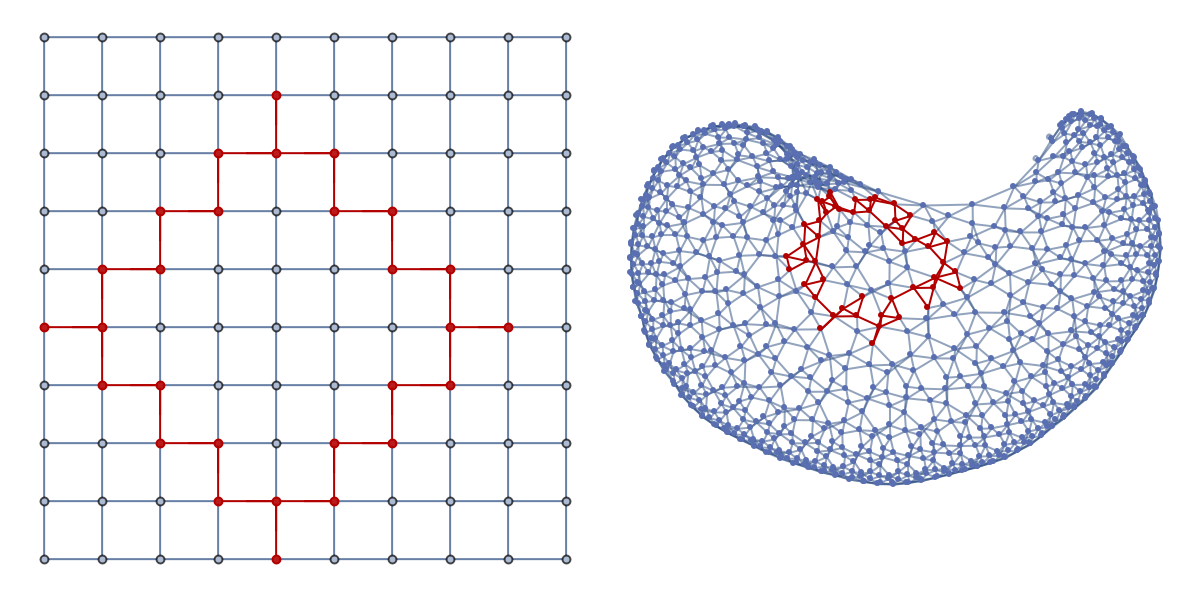
\includegraphics[width=\linewidth]{shell.png}
        \caption{Graph-distance shell.}
        \label{fig:shell}
    \end{subfigure}
    \hfill
    \begin{subfigure}{0.48\linewidth}
        \centering
        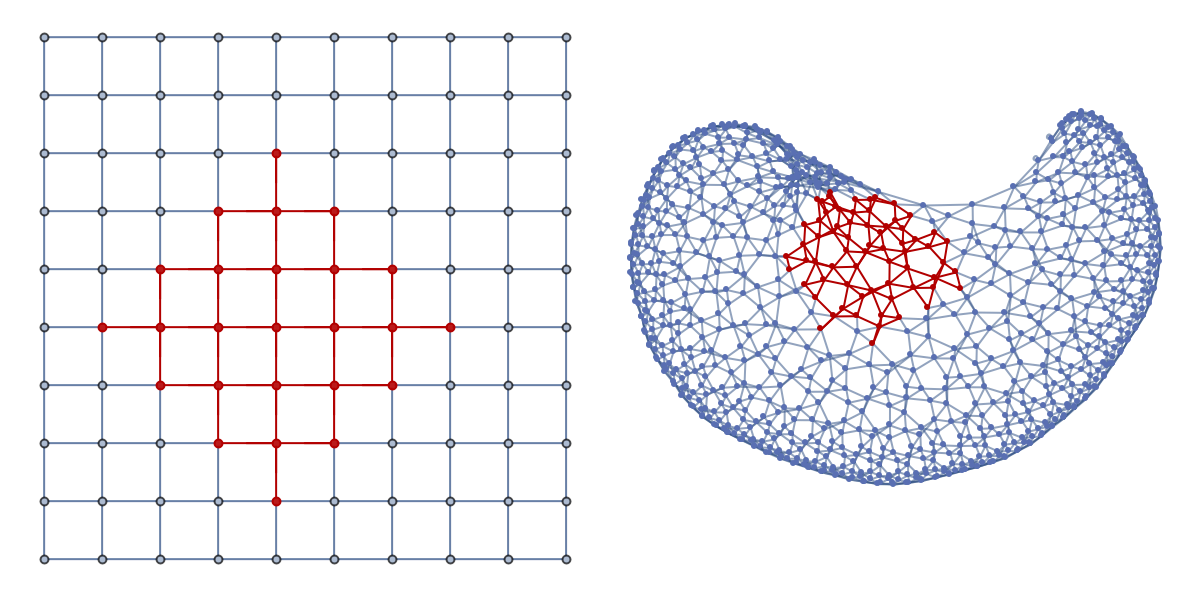
\includegraphics[width=\linewidth]{ball.png}
        \caption{Graph-distance ball.}
        \label{fig:ball}
    \end{subfigure}
    \caption{Graph-distance shell and ball used by the estimator. The shell $S_{r_g}(p)$ consists of vertices exactly $r_g$ graph steps away from the center vertex $p$, while the ball $B_{r_g}(p)$ contains all vertices within that graph distance.}
    \label{fig:shell-ball}
\end{figure}

\subsection{Shortest-path count}

For each shell vertex $q\in S_{r_g}(p)$, define $N_{\mathrm{geo}}(p,q)$ as the number of shortest paths from $p$ to $q$.

\subsection{Path-anisotropy estimator}

The current main estimator is

\begin{equation}
C_{\log}(p,r_g)
=
\mathrm{CMD}_{q\in S_{r_g}(p)}
\left[
\log\left(N_{\mathrm{geo}}(p,q)\right)
\right],
\end{equation}

where $\mathrm{CMD}$ denotes the cubic mean deviation over the shell. In the Mathematica code, this estimator corresponds to the \texttt{LogCMD} column.

\section{Numerical setup}

\subsection{Benchmark geometry}

The main benchmark is a Flamm paraboloid / Schwarzschild spatial-slice-inspired point cloud. For mass $M$, the embedded Flamm surface is sampled using

\begin{equation}
z = 2\sqrt{2M(r-2M)}.
\end{equation}

In the current runs, $M=1/2$, so the inner radius begins slightly above $r=1$. The continuum comparison target is $K_{\mathrm{Schw}}=48M^2/r^6$.

\begin{figure}[H]
    \centering
    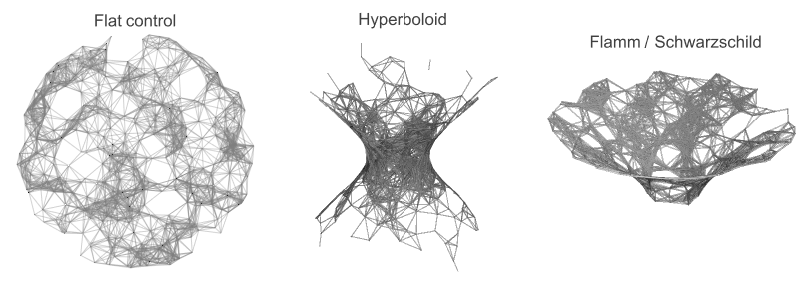
\includegraphics[width=0.9\linewidth]{benchmark_geometries.png}
    \caption{Benchmark point clouds used in the graph-discretization tests. The main benchmark is the Flamm/Schwarzschild spatial-slice-inspired geometry, with flat and hyperboloid-like geometries used as controls or additional test cases.}
    \label{fig:benchmark-geometries}
\end{figure}

\subsection{Graph construction}

The graph is built using a $k$-nearest-neighbor construction over the sampled embedded points. The current choices are summarized in Table~\ref{tab:kchoices}.

\begin{table}[h]
\centering
\begin{tabular}{cc}
\toprule
$N$ & $k$ \\
\midrule
200 & 12 \\
500 & 14 \\
1000 & 16 \\
\bottomrule
\end{tabular}
\caption{Current graph sizes and $k$-nearest-neighbor parameters.}
\label{tab:kchoices}
\end{table}

The graph radius values studied most carefully are $r_g=3$ and $r_g=4$.

\section{Results so far}

\subsection{Vertex-level convergence with graph refinement}

Multi-seed runs were performed for $N=200,500,1000$. The main statistic is the Spearman rank correlation between the vertex-level estimator $C_{\log}$ and the continuum target $K_{\mathrm{Schw}}$.

\begin{table}[h]
\centering
\begin{tabular}{ccccc}
\toprule
$N$ & graph radius & Mean Pearson & Mean Spearman & Std. Spearman \\
\midrule
200 & 3 & 0.1781 & 0.5320 & 0.1364 \\
200 & 4 & 0.1134 & 0.3346 & 0.1661 \\
500 & 3 & 0.1773 & 0.5630 & 0.0761 \\
500 & 4 & 0.1666 & 0.5023 & 0.0679 \\
1000 & 3 & 0.2460 & 0.6636 & 0.0469 \\
1000 & 4 & 0.2496 & 0.6274 & 0.0553 \\
\bottomrule
\end{tabular}
\caption{Preliminary refinement results for the logarithmic path-anisotropy estimator.}
\label{tab:convergence}
\end{table}

The Spearman correlation increases with graph size, while the standard deviation across random seeds decreases with graph size. The estimator tracks curvature ordering better than raw curvature magnitude. Radius $r_g=3$ is currently the strongest local shell radius, though $r_g=4$ improves significantly at larger $N$.

\begin{figure}[h]
    \centering
    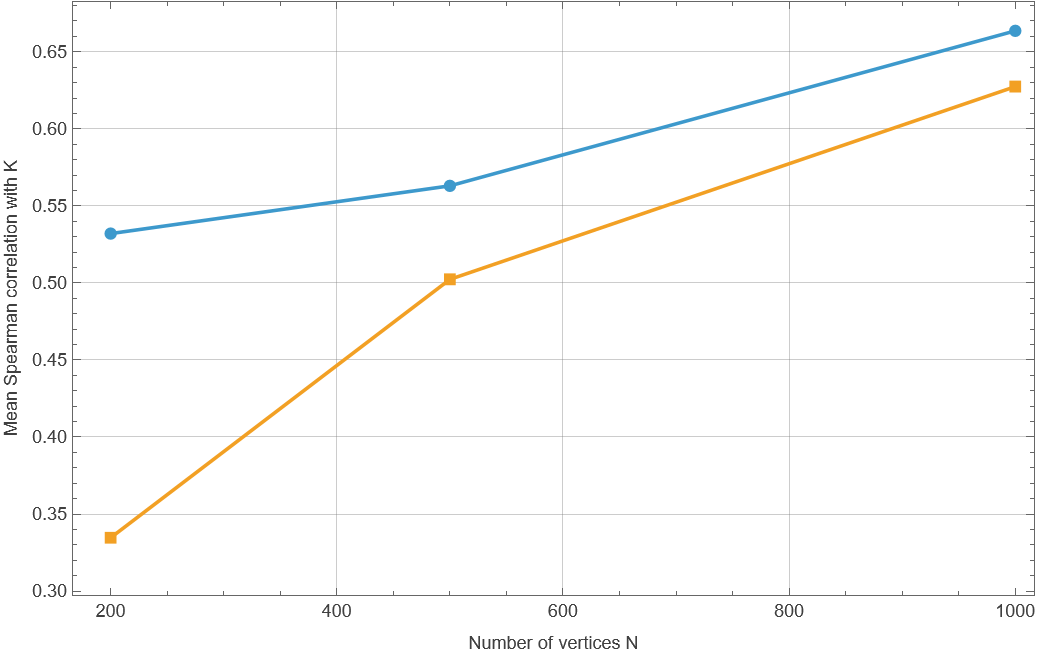
\includegraphics[width=0.85\linewidth]{mean_spearman_vs_N.png}
    \caption{Mean Spearman rank correlation between the logarithmic path-anisotropy estimator and the Schwarzschild Kretschmann scalar. The correlation increases with graph resolution for both graph radii $r_g=3$ and $r_g=4$.}
    \label{fig:mean-spearman}
\end{figure}

\begin{figure}[h]
    \centering
    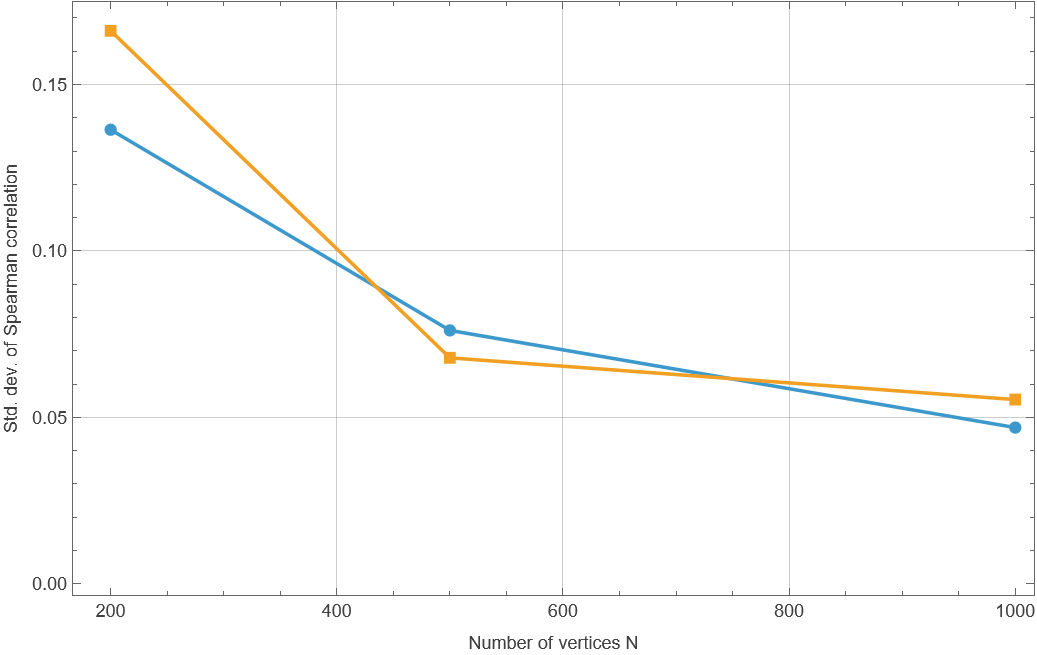
\includegraphics[width=0.85\linewidth]{std_spearman_vs_N.png}
    \caption{Seed-to-seed standard deviation of the Spearman correlation. The decreasing trend suggests improved stability under graph refinement.}
    \label{fig:std-spearman}
\end{figure}

\subsection{Radial binning result}

Since the Schwarzschild Kretschmann scalar depends only on radial coordinate, the vertex-level comparison is noisy. A more physically meaningful comparison groups vertices into radial bins and averages the estimator inside each bin.

For $N=500$, graph radius $r_g=3$, and 12 radial bins, the current run gives

\begin{equation}
\mathrm{Corr}(K_{\mathrm{Schw}}, C_{\log}) \approx 0.497,
\end{equation}

\begin{equation}
\mathrm{Corr}(\log K_{\mathrm{Schw}}, C_{\log}) \approx 0.912,
\end{equation}

and

\begin{equation}
\rho_{\mathrm{Spearman}} \approx 0.874.
\end{equation}

The estimator does not scale linearly with raw $K_{\mathrm{Schw}}$, but it has a strong linear relation with $\log K_{\mathrm{Schw}}$ and a strong monotonic relation with the curvature profile. The estimator also decreases with radial distance, consistent with the expected decrease of Schwarzschild curvature.

\begin{figure}[h]
    \centering
    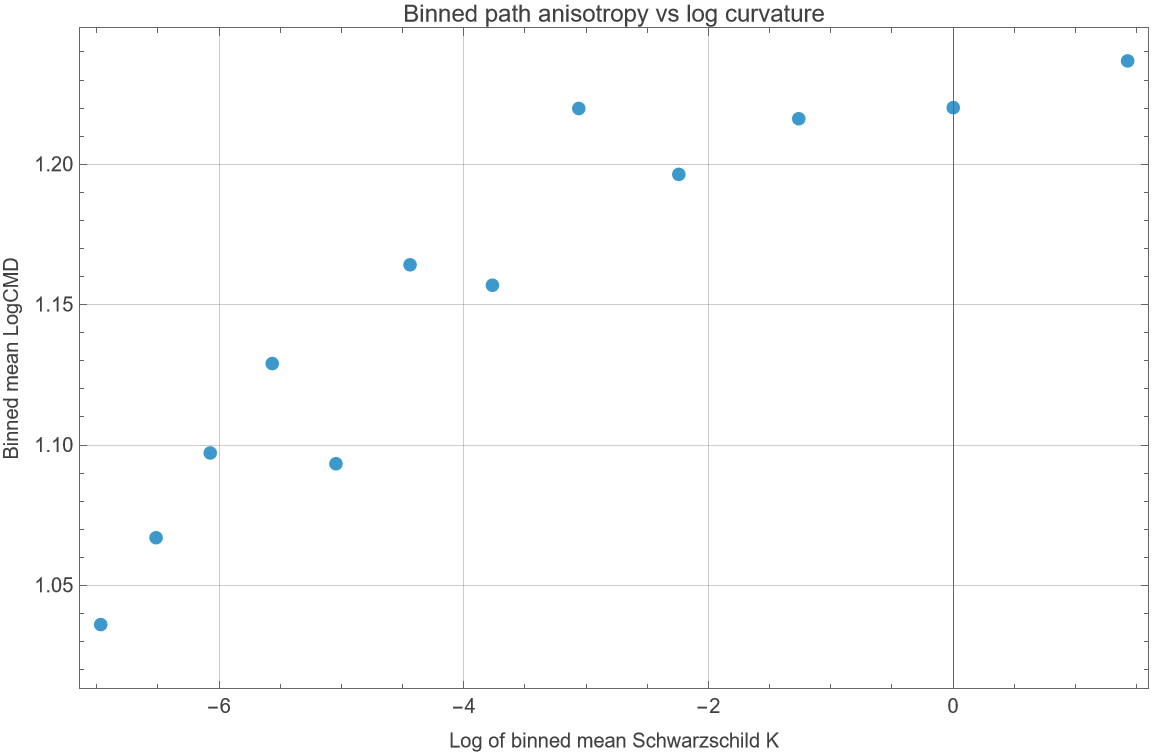
\includegraphics[width=0.85\linewidth]{binned_estimator_vs_logK.png}
    \caption{Radially binned logarithmic path-anisotropy estimator versus $\log K_{\mathrm{Schw}}$. The binned estimator shows a strong positive relation with the logarithmic Schwarzschild curvature profile.}
    \label{fig:binned-logk}
\end{figure}

\begin{figure}[h]
    \centering
    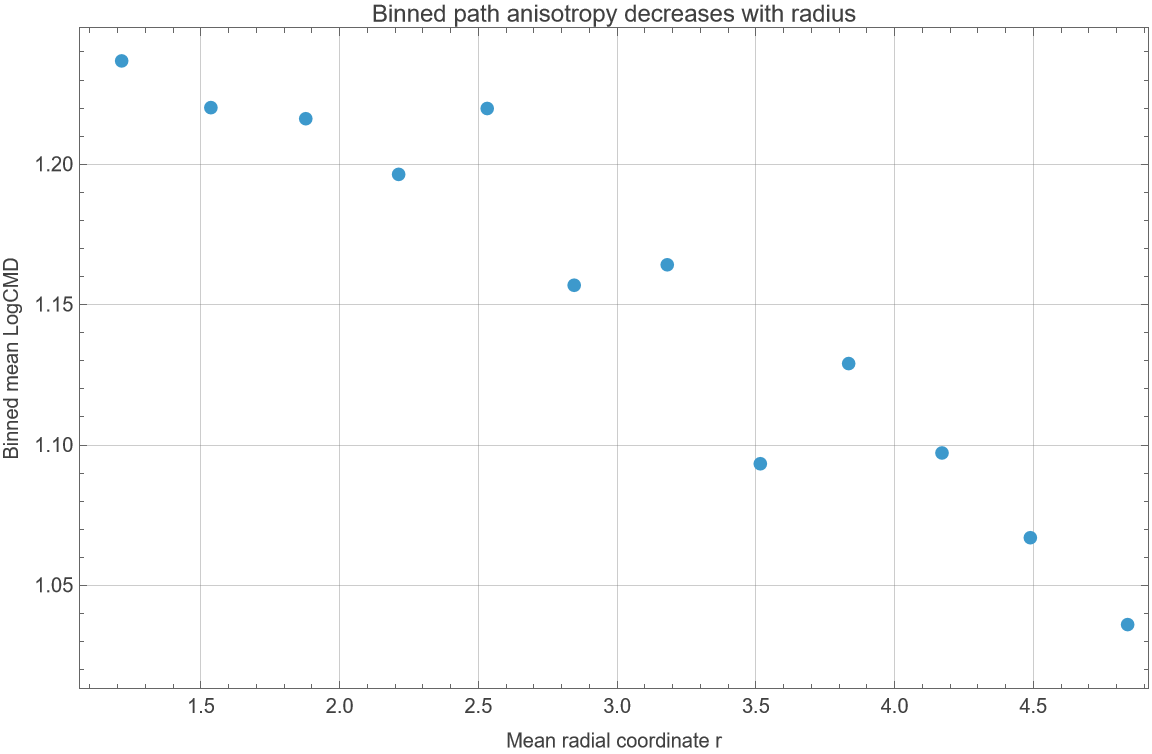
\includegraphics[width=0.85\linewidth]{binned_estimator_vs_r.png}
    \caption{Radially binned logarithmic path-anisotropy estimator as a function of mean radial coordinate. The estimator decreases away from the high-curvature region, consistent with the Schwarzschild curvature profile.}
    \label{fig:binned-r}
\end{figure}

\subsection{Flat-space radial control}

A flat-space control was used to check whether the estimator only separates curved and flat graphs through a simple global shift. The global distributions of \texttt{LogCMD} overlap strongly, with Cohen effect size

\begin{equation}
d_{\mathrm{Cohen}} \approx -0.027.
\end{equation}

The more relevant comparison is radial. In the flat benchmark, the radial correlation between binned mean \texttt{LogCMD} and radial coordinate is close to zero, while the Flamm/Schwarzschild benchmark is strongly negative.

\begin{figure}[H]
    \centering
    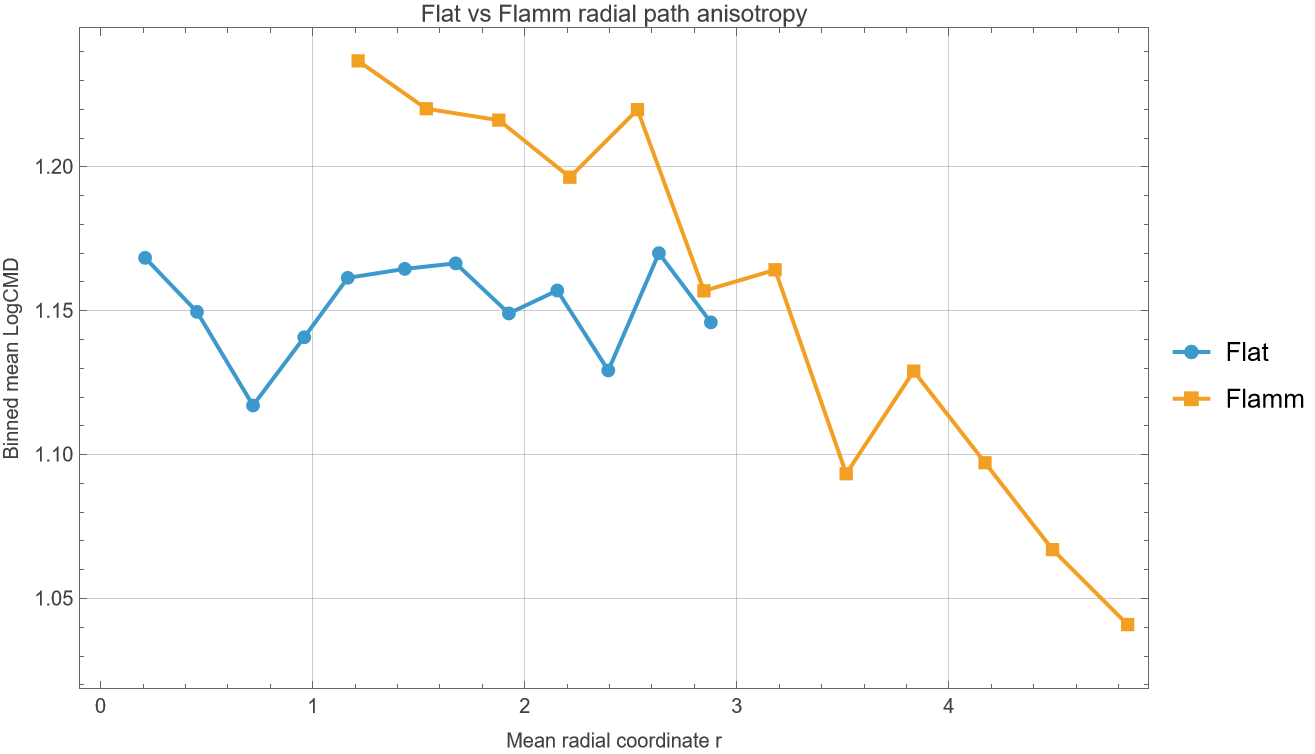
\includegraphics[width=0.85\linewidth]{flat_vs_flamm_radial_logcmd.png}
    \caption{Flat versus Flamm radial path anisotropy. The flat control does not reproduce the strong negative radial trend seen in the Flamm/Schwarzschild benchmark.}
    \label{fig:flat-vs-flamm}
\end{figure}

\subsection{Matched-flat control}

A stronger null test keeps the same radial and angular sampling as the Flamm graph while removing the embedded height profile. The Flamm points

\begin{equation}
(r\cos\theta,r\sin\theta,z(r))
\end{equation}

are replaced by matched-flat points

\begin{equation}
(r\cos\theta,r\sin\theta).
\end{equation}

For $N=1000$, graph radius $r_g=3$, and 12 radial bins, the matched-flat control gives

\begin{equation}
\mathrm{Corr}(r,C_{\log})_{\mathrm{MatchedFlat}} \approx 0.375,
\end{equation}

whereas the Flamm/Schwarzschild benchmark gives

\begin{equation}
\mathrm{Corr}(r,C_{\log})_{\mathrm{Flamm}} \approx -0.985.
\end{equation}

\begin{figure}[H]
    \centering
    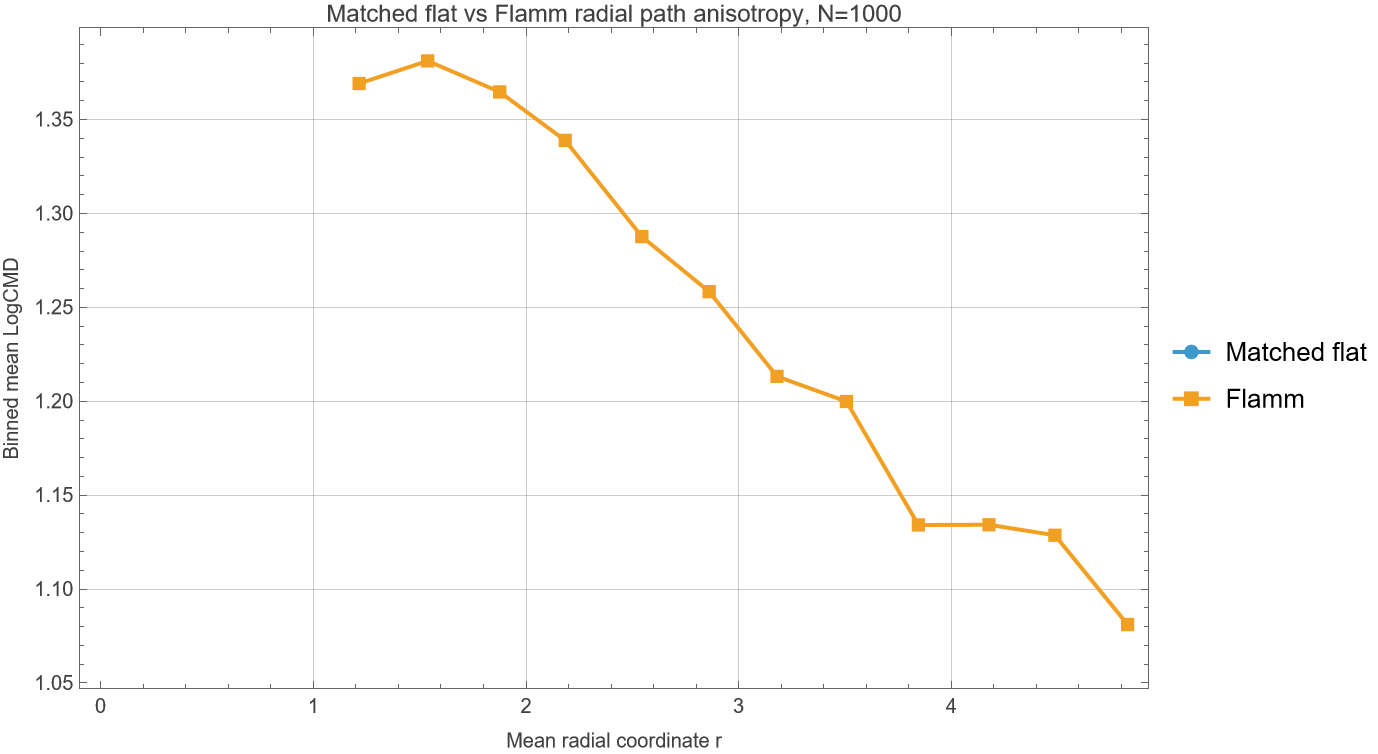
\includegraphics[width=0.85\linewidth]{matched_flat_vs_flamm_radial_logcmd_N1000.png}
    \caption{Matched-flat versus Flamm radial path anisotropy for $N=1000$. The matched-flat control preserves the radial sampling but removes the curved embedding, and it does not reproduce the strong negative Flamm trend.}
    \label{fig:matched-flat-radial}
\end{figure}

Across five random seeds at $N=1000$, $r_g=3$, and $k=16$, the matched-flat control gives

\begin{equation}
\mathrm{Corr}(r,C_{\log})_{\mathrm{MatchedFlat}} = 0.180 \pm 0.315,
\end{equation}

whereas the Flamm benchmark gives

\begin{equation}
\mathrm{Corr}(r,C_{\log})_{\mathrm{Flamm}} = -0.960 \pm 0.015.
\end{equation}

\begin{figure}[H]
    \centering
    \begin{subfigure}{0.48\linewidth}
        \centering
        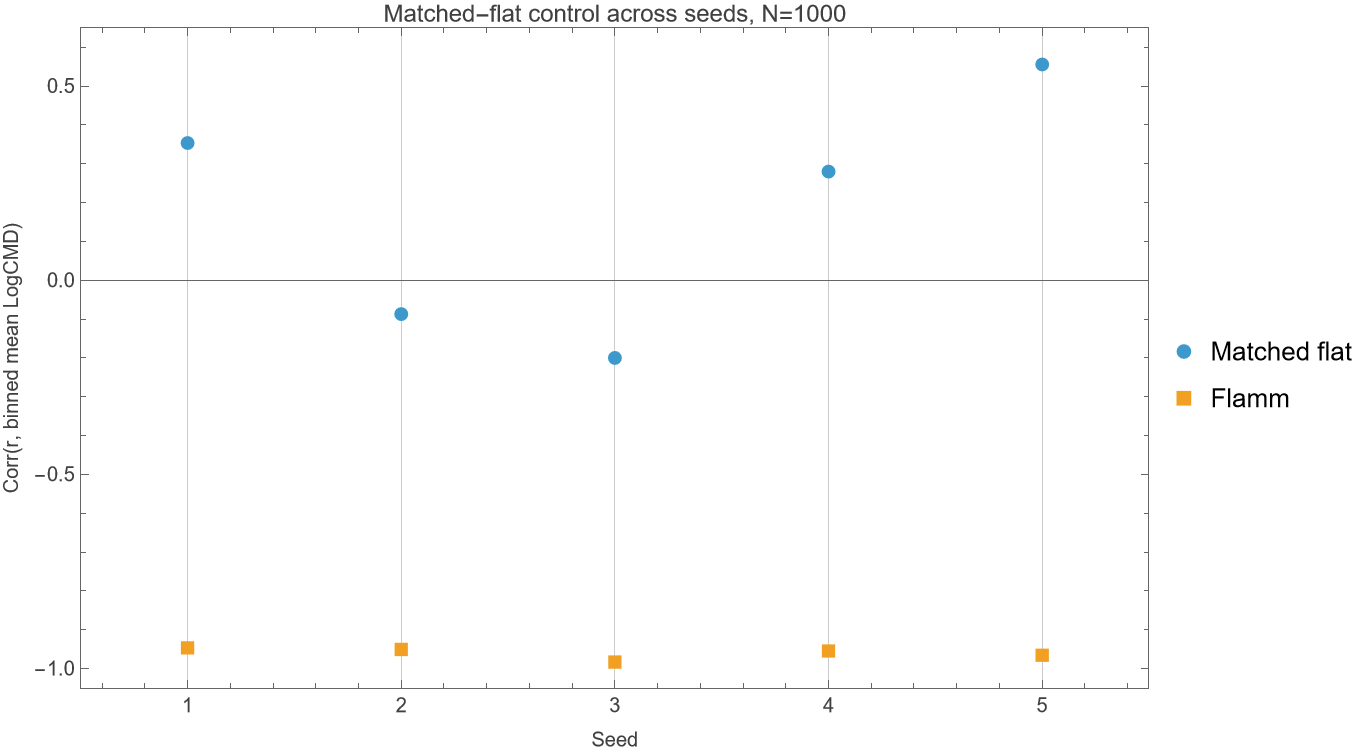
\includegraphics[width=\linewidth]{matched_flat_flamm_seed_scatter_N1000.png}
        \caption{Seed-by-seed correlations.}
        \label{fig:matched-seeds-scatter}
    \end{subfigure}
    \hfill
    \begin{subfigure}{0.48\linewidth}
        \centering
        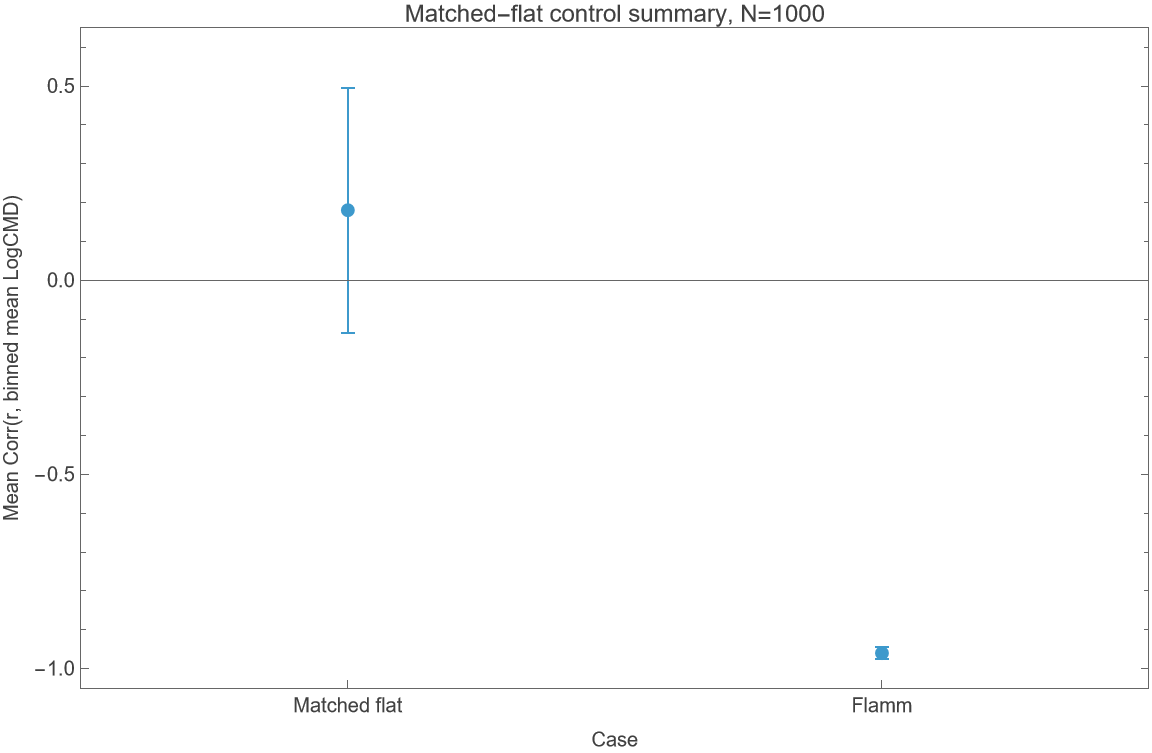
\includegraphics[width=\linewidth]{matched_flat_flamm_summary_N1000.png}
        \caption{Mean and standard deviation.}
        \label{fig:matched-seeds-summary}
    \end{subfigure}
    \caption{Matched-flat control across five random seeds. The Flamm/Schwarzschild benchmark is stably and strongly negatively correlated with radial coordinate, while the matched-flat control is variable and not consistently negative.}
    \label{fig:matched-flat-seeds}
\end{figure}

\subsection{$k$-sensitivity}

To test dependence on graph construction, the matched-flat and Flamm comparisons were repeated for several $k$-nearest-neighbor values. For $N=1000$, $r_g=3$, 12 radial bins, and three random seeds per value of $k$, the results are:

\begin{table}[H]
\centering
\begin{tabular}{rrrrr}
\toprule
$k$ & Matched-flat mean & Matched-flat std & Flamm mean & Flamm std \\n\midrule
12 & 0.125 & 0.330 & -0.942 & 0.016 \\n14 & 0.155 & 0.510 & -0.961 & 0.027 \\n16 & 0.022 & 0.292 & -0.960 & 0.020 \\n18 & 0.165 & 0.413 & -0.965 & 0.018 \\n20 & 0.372 & 0.166 & -0.962 & 0.023 \\n\bottomrule
\end{tabular}
\caption{$k$-sensitivity of the matched-flat and Flamm radial correlations. The Flamm signal remains strongly negative across the tested graph connectivities.}
\label{tab:k-sensitivity}
\end{table}

\begin{figure}[H]
    \centering
    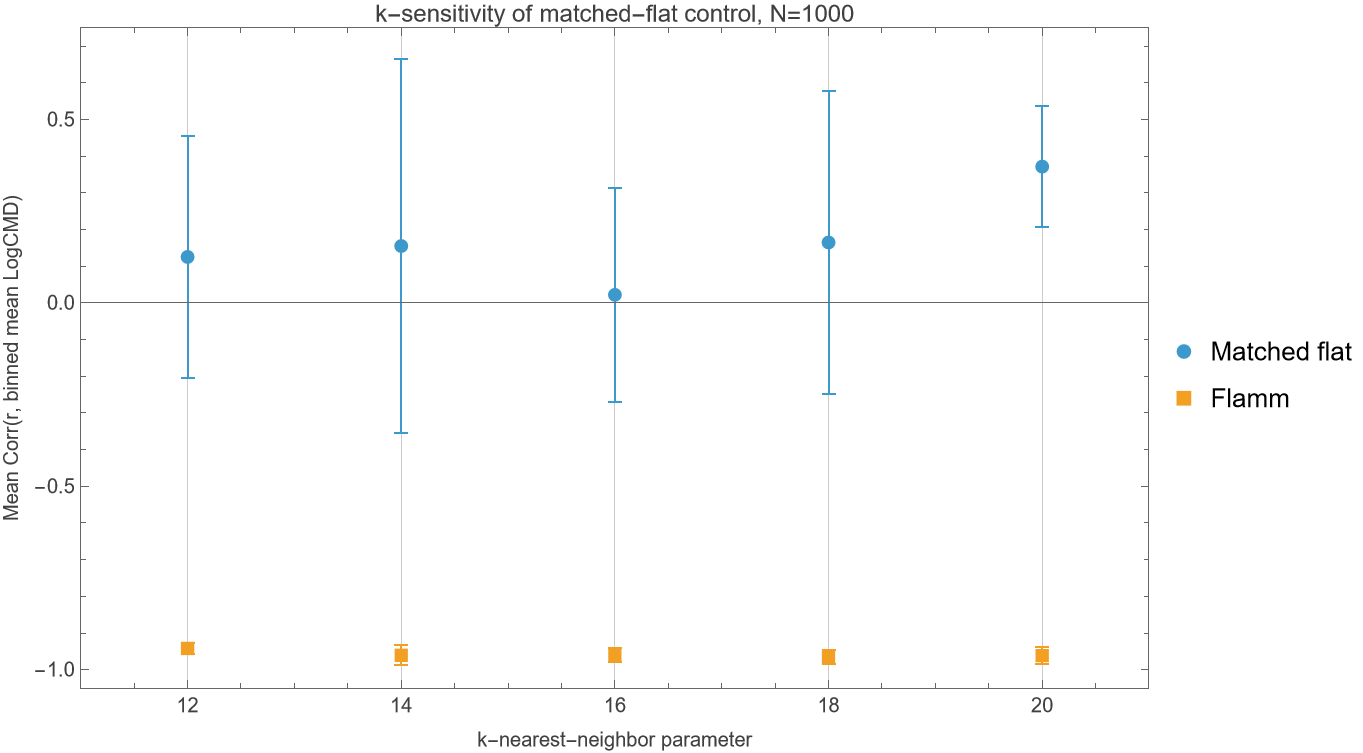
\includegraphics[width=0.85\linewidth]{k_sensitivity_matched_flat_flamm_N1000_errors.png}
    \caption{$k$-sensitivity of the matched-flat control and Flamm benchmark. Error bars show seed-to-seed standard deviation over three random seeds for each $k$.}
    \label{fig:k-sensitivity}
\end{figure}

\section{Possible paper structure}

\subsection{Introduction}

The introduction should explain why curvature diagnostics are important in discrete geometries, mention graph/hypergraph/discrete spacetime motivation, introduce the challenge that there is no direct smooth Riemann tensor in a graph, and state the idea of using shortest-path anisotropy over graph-distance shells.

\subsection{Background}

The background should discuss continuum curvature and the Kretschmann scalar, the Schwarzschild benchmark $K_{\mathrm{Schw}}=48M^2/r^6$, and existing discrete curvature approaches such as Ollivier-Ricci curvature, Forman-Ricci curvature, causal-set scalar curvature, Wolfram-model curvature constructions, and recent path-count/Weyl-type causal-set estimators. The present estimator differs because it uses shortest-path-count variation over graph shells.

\subsection{Path-anisotropy estimator}

This section should define $B_{r_g}(p)$, $S_{r_g}(p)$, and $N_{\mathrm{geo}}(p,q)$, then introduce \texttt{OldCMD}, \texttt{NormalizedCMD}, and \texttt{LogCMD}. The main text should explain why \texttt{LogCMD} is used as the primary estimator: shortest-path counts can grow quickly, and the logarithm stabilizes the scale.

\subsection{Benchmark construction}

This section should describe Flamm surface sampling, the $k$-nearest-neighbor graph construction, the target curvature $K_{\mathrm{Schw}}$, random seed averaging, and graph refinement.

\subsection{Results}

The results section should show the benchmark geometry image, the mean Spearman convergence plot, the standard-deviation plot, the binned estimator versus $\log K$, and the binned estimator versus radial coordinate.

\subsection{Discussion}

The discussion should emphasize that the estimator tracks curvature ordering, not direct magnitude; radial binning reveals a clearer curvature profile; the signal strengthens under graph refinement; and the valid shell radius appears local. Boundary effects and graph construction choices matter.

\subsection{Limitations and next work}

The estimator is not yet a discrete Kretschmann scalar and is not a tensor reconstruction. The next steps are flat null tests, additional curved benchmarks, sensitivity tests with respect to $k$, comparison with existing graph curvature definitions, and extension to hypergraphs and evolved Wolfram-model states.

\section{Limitations}

The strongest limitation is conceptual: the estimator is not derived from a discrete Riemann tensor. It is a path-statistical diagnostic.

Other limitations are:

\begin{itemize}
    \item Current results use graph discretizations, not full hypergraph evolution.
    \item The Flamm benchmark is a spatial slice, not a full Lorentzian spacetime.
    \item The estimator is sensitive to graph construction choices.
    \item Raw vertex-level correlations are moderate; radial binning gives a stronger signal.
    \item The estimator appears to track $\log K$ better than $K$.
\end{itemize}

\section{Next experiments}

Immediate steps:

\begin{enumerate}
    \item Upload the current repository and figures.
    \item Export the convergence and binned tables as CSV.
    \item Add a flat-space null test.
    \item Add plots for the flat control.
\end{enumerate}

Near-term steps:

\begin{enumerate}
    \item Repeat radial binning for $N=1000$.
    \item Test $k=10,12,14,16,18$.
    \item Test graph radii $r_g=2,3,4,5$.
    \item Add hyperboloid/sphere controls.
    \item Compare \texttt{OldCMD}, \texttt{NormalizedCMD}, and \texttt{LogCMD}.
\end{enumerate}

Paper-strength tests:

\begin{enumerate}
    \item Show the signal is absent or much weaker in flat controls.
    \item Show the signal survives multiple graph construction choices.
    \item Show the signal improves under refinement.
    \item Compare against at least one existing graph curvature measure.
    \item Formulate a careful continuum-limit conjecture.
\end{enumerate}

\section{Current best wording}

Good cautious wording:

\begin{quote}
We introduce a local path-anisotropy observable based on shortest-path counts over graph-distance shells and test it as a curvature diagnostic in graph discretizations of continuum geometries.
\end{quote}

Good result wording:

\begin{quote}
In the Flamm/Schwarzschild benchmark, the logarithmic path-anisotropy estimator shows a positive rank correlation with the continuum Kretschmann profile. The correlation strengthens and becomes less seed-dependent under graph refinement. After radial binning, the estimator has a strong correlation with $\log K_{\mathrm{Schw}}$.
\end{quote}

Avoid saying:

\begin{quote}
We define the Kretschmann scalar for hypergraphs.
\end{quote}

Safer alternative:

\begin{quote}
We study a Kretschmann-inspired curvature diagnostic for graph and hypergraph discretizations.
\end{quote}

\end{document}
